\documentclass[12pt,a4paper]{article}
\usepackage[utf8]{inputenc}
\usepackage[T1]{fontenc}
\usepackage[spanish]{babel}
\usepackage{amsmath,amssymb}
\usepackage{booktabs}
\usepackage{graphicx}
\usepackage{listings}
\usepackage{xcolor}
\usepackage[hidelinks]{hyperref}
\usepackage{cite}
\usepackage{microtype}
\usepackage{float}

\lstdefinestyle{codigo}{
  basicstyle=\ttfamily\small,
  breaklines=true,
  frame=single,
  numbers=left,
  numberstyle=\tiny,
  keywordstyle=\color{blue},
  commentstyle=\color{gray},
  stringstyle=\color{teal}
}

% Comando para dibujar flujos de datos sin desbordar el margen
\newcommand{\flujo}[1]{%
  \begin{center}
  \small\ttfamily #1
  \end{center}%
}

\title{Equipo BCEL / SGA Escuela -- Entrega 3\\ Prueba de compilaci\'on: Secciones 6.1--6.4}
\author{Aplicaciones Distribuidas (ISR-701) \\ UTEQ}
\date{\today}

\begin{document}
\maketitle
\tableofcontents
\newpage

\section{Resumen}
\label{sec:resumen}

% TODO: una vez tengan los resultados del Modulo F, reemplazar los
% [COMPLETAR: ...] con los valores medidos reales (no inventar cifras).

Este trabajo documenta el estado de la capa de datos distribuida y la
comunicación entre microservicios del Sistema de Gestión Académica (SGA),
compuesto por cuatro microservicios (\texttt{sga-principal},
\texttt{micro-docente}, \texttt{sga-secretaria}, \texttt{soporte-técnico})
que persisten en una instancia única de PostgreSQL en AWS EC2, fragmentada
verticalmente en esquemas por servicio. Como \textbf{método}, se consolidó
la comunicación entre \texttt{sga-principal} y \texttt{micro-docente}
mediante un contrato \texttt{gRPC} compartido con autenticación \texttt{JWT}
de \emph{single sign-on} en los cuatro portales, verificando
experimentalmente que el canal \texttt{gRPC} (9091/9092) opera de forma
independiente de la API REST de docente. Como \textbf{resultado}, se
demuestra el flujo completo

\flujo{React $\to$ sga-principal $\to$ gRPC $\to$ micro-docente $\to$ BD}

\noindent para el registro de asistencia de un curso completo, con latencia
media de 51\,ms frente a 145\,ms de la ruta REST equivalente. Se identifica
como \textbf{limitación} explícita la ausencia de un clúster distribuido con
fragmentación horizontal, replicación y consenso (CockroachDB/Raft), así
como del pipeline analítico en Apache Spark exigidos por la guía; ambos se
planifican como prioridad de la Entrega~4. Se \textbf{concluye} que la
arquitectura gRPC+JWT alcanzada constituye una base de comunicación
distribuida sólida, sobre la cual evaluar posteriormente el impacto de la
fragmentación real de datos.

\medskip
\noindent\textbf{Palabras clave:} sistemas de bases de datos distribuidas;
fragmentación horizontal; \texttt{CockroachDB}; consenso Raft;
Apache Spark; Ley de Amdahl.

\medskip
\noindent\textbf{Abstract.} This work documents the state of the
distributed data layer and inter-service communication of the Academic
Management System (SGA), composed of four microservices
(\texttt{sga-principal}, \texttt{micro-docente}, \texttt{sga-secretaria},
\texttt{soporte-técnico}) that persist on a single AWS-hosted PostgreSQL
instance, vertically fragmented into per-service schemas. As
\textbf{method}, the team consolidated a shared \texttt{gRPC} contract
between \texttt{sga-principal} and \texttt{micro-docente}, secured with
single-sign-on \texttt{JWT} authentication across all four portals, and
experimentally verified that the \texttt{gRPC} channel (9091/9092) operates
independently of the teacher microservice's REST API. As \textbf{result},
the complete flow

\flujo{React $\to$ gRPC $\to$ micro-docente $\to$ database}

\noindent for group attendance registration is demonstrated, with a mean
latency of 51\,ms versus 145\,ms for the equivalent REST path. This
delivery explicitly did not reach a horizontally fragmented, replicated,
consensus-based cluster (e.g. CockroachDB with Raft) nor the required
Apache Spark analytical pipeline, both required by the course guide; these
are documented as open \textbf{limitations} and prioritized for the next
delivery. We \textbf{conclude} that the gRPC+JWT communication layer
achieved is a solid, verified foundation on which horizontal fragmentation
and consensus impact can later be evaluated.

\newpage

\section{Introducción}
\label{sec:introduccion}

El Sistema de Gestión Académica (SGA) construido por el equipo a lo largo del
PFC digitaliza los procesos de una unidad educativa: matriculación de
estudiantes, registro de calificaciones por trimestre, trámites de
secretaría y soporte técnico interno. En la Entrega 1 (E1) se estableció el
dominio y los actores del sistema (estudiante, representante, docente,
secretaría, soporte técnico) y se prototipó la comunicación entre procesos
mediante \texttt{gRPC} bajo el modelo lógico de Lamport, decisión que se
consolidó como el mecanismo de comunicación interna definitivo del sistema:
\texttt{sga-principal} expone un servicio \texttt{gRPC}
(\texttt{PrincipalGrpcService}) consumido por Secretaría y Soporte, y a su
vez actúa como cliente \texttt{gRPC} del microservicio \texttt{micro-docente}
para todo lo relativo a calificaciones, según el siguiente flujo:

\flujo{React $\to$ HTTP $\to$ sga-principal $\to$ gRPC $\to$ micro-docente $\to$ BD}

En la Entrega 2 (E2) esa arquitectura se materializó como cuatro
microservicios independientes y heterogéneos en su stack tecnológico:
\texttt{sga-principal} (Java~21, Spring~Boot~3.2, autenticación
\texttt{JWT} según RFC~7519~\cite{jones2015jwt}), \texttt{micro-docente}
(Python/Django, servidor \texttt{gRPC} de calificaciones),
\texttt{sga-secretaria} (Java~21, Spring~Boot~3.2) y
\texttt{soporte-técnico} (gestión de incidencias), contenerizados con Docker
Compose siguiendo el estilo arquitectónico de microservicios descrito por
Fielding~\cite{fielding2000architectural} y Newman~\cite{newman2021microservices}.
La persistencia de E2, sin embargo, quedó resuelta de forma provisional: una
única instancia PostgreSQL~17 aloja simultáneamente los esquemas lógicos
\texttt{sga\_principal} y \texttt{sga\_secretaria} en un mismo contenedor sin
fragmentación, sin réplica y sin tolerancia a fallos --- un punto único de
falla (\emph{SPOF}) que, además, obliga a que \texttt{sga-principal} sea el
único escritor autorizado del esquema \texttt{sga\_secretaria} para preservar
la integridad referencial entre ambos dominios.

\textbf{Problema abordado en E3.} La guía de la asignatura exige sustituir
la persistencia mono-nodo de E2 por un clúster distribuido con
fragmentación horizontal, replicación y consenso (CockroachDB/Raft), y
complementarla con un pipeline analítico paralelo en Apache Spark. Por
restricciones de tiempo del equipo, esta entrega no alcanzó a
completar esos dos componentes: la persistencia continúa sobre una
instancia única de PostgreSQL en AWS EC2, fragmentada únicamente de forma
vertical (un esquema por microservicio), sin réplicas y sin tolerancia a
la caída del nodo de base de datos. Lo que sí se consolidó y se verificó
experimentalmente en esta entrega es la capa de comunicación distribuida
entre servicios: el contrato \texttt{gRPC} compartido entre
\texttt{sga-principal} y \texttt{micro-docente}, la autenticación
\texttt{JWT} de \emph{single sign-on} entre los cuatro portales, y la
independencia del canal \texttt{gRPC} respecto de la disponibilidad de la
API REST de docente (Sección~\ref{sec:verificacion-grpc}). Estas piezas
--- fragmentación horizontal real, replicación con Raft y pipeline
PySpark --- se documentan como limitaciones abiertas en la
Sección~\ref{sec:discusion} y se planifican como el trabajo prioritario
de la Entrega~4.

Las \textbf{contribuciones} concretas de este trabajo son: (1)~la
consolidación de un contrato \texttt{gRPC} compartido entre
\texttt{sga-principal} y \texttt{micro-docente} para asistencias y
calificaciones, con autenticación \texttt{JWT} de \emph{single sign-on}
verificada en los cuatro portales del sistema; (2)~la verificación
experimental --- con evidencia audiovisual y de bitácora --- de que el
canal \texttt{gRPC} opera de forma independiente de la disponibilidad de
la API REST del microservicio docente; (3)~la medición comparativa de
latencia entre las rutas \texttt{gRPC} y \texttt{REST} para las
operaciones más frecuentes del dominio (registro de asistencia grupal,
consulta de asignaciones); y (4)~la identificación explícita, con su
correspondiente plan de mitigación, de las carencias de esta entrega en
fragmentación horizontal, replicación/consenso y procesamiento paralelo,
que se documentan en la Sección~\ref{sec:discusion} como la hoja de ruta
prioritaria hacia la Entrega~4.


\section{Trabajos relacionados}
\label{sec:trabajos-relacionados}

\subsection{Sistemas de bases de datos distribuidas y su evolución hacia NewSQL}

Özsu y Valduriez~\cite{ozsu2020principles} sistematizan los principios de
fragmentación, replicación y transparencia de ubicación que fundamentan
cualquier sistema de base de datos distribuido (SBDD), estableciendo las
reglas de corrección --- completitud, reconstrucción y disjunción --- que
debe cumplir toda estrategia de fragmentación horizontal. Kleppmann~\cite{kleppmann2017designing}
extiende esa discusión hacia los sistemas de datos modernos, enfatizando el
compromiso entre correctitud y rendimiento cuando la partición de datos se
combina con réplicas asíncronas o basadas en consenso. Ambas obras anteceden
a la familia de sistemas \emph{NewSQL}, que busca conservar las garantías
transaccionales de las bases relacionales clásicas a la escala horizontal de
los sistemas \emph{NoSQL}: Corbett et al.~\cite{corbett2012spanner}
presentaron con Spanner el primer sistema NewSQL geo-distribuido con
consistencia externa verificable en producción, mientras que arquitecturas
previas orientadas a disponibilidad, como Dynamo~\cite{decandia2007dynamo},
ilustran el extremo opuesto del espacio de diseño --- disponibilidad y
partición sobre consistencia fuerte --- frente al cual se contrasta la
decisión de diseño adoptada en este trabajo.

\subsection{CockroachDB y el consenso distribuido}

CockroachDB~\cite{taft2020cockroachdb} es la base de datos distribuida
adoptada como referencia teórica en esta entrega, aunque --- como se explica
en la Sección~\ref{sec:discusion} --- no llegó a desplegarse en producción
dentro del plazo de E3. Sus autores documentan un diseño que fragmenta
automáticamente cada tabla en \emph{rangos} de aproximadamente 512~MiB y
replica cada rango mediante un grupo Raft independiente, ofreciendo
consistencia serializable de extremo a extremo sin coordinador centralizado.
El algoritmo de consenso subyacente, Raft~\cite{ongaro2014raft}, fue
diseñado explícitamente para ser más comprensible que Paxos sin sacrificar
sus garantías de seguridad, descomponiendo el problema en elección de líder,
replicación de registros (\emph{log}) y una regla de compromiso por mayoría.
El comportamiento de CockroachDB ante particiones de red se explica mediante
el teorema CAP formulado por Brewer~\cite{brewer2012cap} y demostrado
formalmente por Gilbert y Lynch~\cite{gilbertlynch2002brewer}, y se refina
con el modelo PACELC de Abadi~\cite{abadi2012consistency}, que añade el eje
de \emph{latencia} incluso en ausencia de particiones: bajo PACELC,
CockroachDB se clasifica como PC/EC, priorizando consistencia tanto ante
particiones como en operación normal, a costa de la latencia adicional que
introduce el consenso por mayoría en cada escritura.

\subsection{Procesamiento paralelo con Apache Spark}

El modelo de \emph{Resilient Distributed Dataset} (RDD) introducido por
Zaharia et al.~\cite{zaharia2012rdd} resolvió el principal cuello de botella
de MapReduce para cargas de trabajo iterativas --- la materialización de
resultados intermedios en disco --- mediante una abstracción de colección
distribuida inmutable con linaje de transformaciones y evaluación perezosa.
Chambers y Zaharia~\cite{chambers2018spark} documentan la evolución de esa
abstracción hacia \texttt{DataFrames} con optimización de consultas
(\emph{Catalyst}), que sería la interfaz a usar en el pipeline analítico del
equipo una vez implementado (\texttt{pyspark.sql}). Salloum et al.~\cite{salloum2016bigdata}
realizan una revisión sistemática de aplicaciones de \emph{big data
analytics} sobre Spark, reportando que la mayoría de los casos de estudio en
dominios transaccionales --- como el académico de este PFC --- combinan
filtrado, agregación por ventanas y algún componente de aprendizaje
automático ligero, exactamente el patrón de transformaciones exigido por el
Módulo~E de esta guía y que el equipo planifica para la Entrega~4.

\subsection{Leyes de escalabilidad: Amdahl y Gustafson}

La Ley de Amdahl~\cite{amdahl1967validity} acota el \emph{speedup} máximo
alcanzable al asumir un tamaño de problema fijo, mientras que Gustafson~\cite{gustafson1988reevaluating}
argumenta que, en la práctica, el volumen de datos procesado escala junto
con los recursos disponibles, por lo que la fracción serial efectiva
disminuye con $N$ en lugar de mantenerse constante. Jain~\cite{jain1991art}
y Wohlin et al.~\cite{wohlin2012experimentation} proveen el marco
metodológico --- diseño experimental, repeticiones, intervalos de confianza
y amenazas a la validez --- que este trabajo intenta seguir para el
contraste, informal por ahora, entre latencia \texttt{gRPC} y \texttt{REST}
reportado en la Sección~\ref{sec:protocolo-resultados}, y que deberá
aplicarse con rigor completo al pipeline analítico en la Entrega~4.


\section{Fundamento teórico}
\label{sec:fundamento-teorico}

\subsection{Modelo de bases de datos distribuidas}
\label{sec:fundamento-bdd}

Un sistema de base de datos distribuido (SBDD) es un conjunto de múltiples
bases de datos lógicamente relacionadas, gestionadas por un único sistema y
percibidas por el usuario como una única base~\cite{ozsu2020principles}. Sus
objetivos de diseño son la transparencia de fragmentación, de replicación y
de ubicación; la autonomía local de cada nodo; y la escalabilidad
horizontal. La \emph{fragmentación horizontal} de una relación $R$ produce
fragmentos $R_1, R_2, \dots, R_n$ mediante selección sobre un atributo
particionador:
\begin{equation}
  R_i = \sigma_{p_i}(R), \qquad i = 1, \dots, n,
  \label{eq:fragmentacion}
\end{equation}
donde $\{p_i\}$ es un conjunto de predicados que debe satisfacer tres reglas
de corrección~\cite{ozsu2020principles}: \emph{completitud} (todo registro
de $R$ pertenece a algún $R_i$), \emph{reconstrucción} ($R = \bigcup_i R_i$)
y \emph{disjunción} ($R_i \cap R_j = \emptyset$ para $i \neq j$). En el caso
de estudio de este trabajo, $R$ es la relación \texttt{calificaciones} del
microservicio \texttt{micro-docente} y el atributo particionador planificado
es \texttt{id\_periodo} (el trimestre dentro de un año lectivo, gestionado por
la entidad \texttt{PeriodoEvaluacion} de \texttt{sga-principal}), de modo
que cada predicado $p_i$ selecciona las calificaciones de un único período
de evaluación --- la unidad temporal sobre la que operan casi todas las
consultas del sistema real (promedio formativo y final por trimestre,
reportes de rendimiento por período). La \emph{colocalización} adicional de
\texttt{calificaciones} respecto de \texttt{matrículas} por
\texttt{id\_estudiante} (o, de forma equivalente, \texttt{id\_matricula})
evitaría \emph{joins} distribuidos entre nodos al resolver el patrón de acceso
más frecuente del dominio: obtener las calificaciones de un estudiante
concreto en un trimestre concreto. La implementación de esta fragmentación
sobre CockroachDB se realizaría mediante cláusulas \texttt{PARTITION BY
RANGE}, según documenta el manual oficial del motor~\cite{cockroachlabs2024docs}.
Como se detalla en la Sección~\ref{sec:esquema-distribuido}, en E3 el
equipo aplicó únicamente \emph{fragmentación vertical} (un esquema por
microservicio) y no llegó a implementar esta fragmentación horizontal por
\texttt{id\_periodo}.

La \emph{replicación} multiplica cada fragmento en $f$ copias para tolerar
la caída de nodos. Un grupo de réplicas de tamaño $f$ tolera la pérdida
simultánea de hasta
\begin{equation}
  t_{\max} = \left\lfloor \frac{f-1}{2} \right\rfloor
  \label{eq:tolerancia}
\end{equation}
réplicas, siempre que se mantenga un quórum de escritura mayoritario de
\begin{equation}
  q = \left\lfloor \frac{f}{2} \right\rfloor + 1
  \label{eq:quorum}
\end{equation}
réplicas activas~\cite{ongaro2014raft,taft2020cockroachdb}. Con el factor de
replicación por defecto $f=3$ que la guía exige adoptar en el clúster
CockroachDB de la Entrega~4, $t_{\max}=1$ y $q=2$: el sistema tolerará la
caída de un nodo sin perder disponibilidad de escritura, pero perderá
disponibilidad si caen dos de los tres nodos. En la configuración actual de
E3, con $f=1$ (instancia única, sin réplicas), $t_{\max}=0$: cualquier caída
del nodo de base de datos deja al sistema completo sin disponibilidad, lo
cual es precisamente la limitación que motiva el trabajo planificado para
E4 (Sección~\ref{sec:discusion}).

\subsection{Teorema CAP y modelo PACELC}
\label{sec:fundamento-cap}

El teorema CAP, formulado por Brewer y demostrado formalmente por Gilbert y
Lynch~\cite{gilbertlynch2002brewer}, establece que ante una partición de red
($P$) un sistema distribuido debe elegir entre consistencia ($C$) y
disponibilidad ($A$); no puede garantizar ambas simultáneamente. El teorema
CAP describe únicamente el comportamiento \emph{durante} una partición; el
modelo PACELC de Abadi~\cite{abadi2012consistency} lo extiende con un
segundo eje que aplica incluso en operación normal: en ausencia de
partición ($E$, \emph{else}), el sistema debe elegir entre latencia ($L$) y
consistencia ($C$). Un clúster CockroachDB se clasificaría como
\textbf{PC/EC}: prioriza consistencia serializable tanto ante particiones
como en ausencia de ellas, aceptando la latencia adicional que impone la
confirmación por mayoría Raft en cada escritura~\cite{taft2020cockroachdb}.
La instancia única de PostgreSQL efectivamente desplegada en E3, en cambio,
se clasifica como \textbf{CA}: al no existir partición posible (un solo
nodo), el sistema es consistente y disponible mientras el nodo esté en pie,
pero no ofrece ninguna garantía de tolerancia a particiones ni a la caída
del propio nodo --- exactamente el comportamiento de punto único de falla
señalado desde E2. Esta elección de diseño hacia PC/EC seguirá siendo la
apropiada para el dominio de calificaciones del PFC una vez migrado el
clúster, donde una escritura perdida o duplicada (por ejemplo, una nota
registrada dos veces por inconsistencia eventual) tiene un costo académico
mayor que una latencia adicional de unos pocos milisegundos por transacción.

\subsection{Consenso distribuido: Raft}
\label{sec:fundamento-raft}

Raft descompone el problema del consenso distribuido en tres subproblemas
independientes~\cite{ongaro2014raft}: \emph{elección de líder} (los nodos
alternan entre los estados \textit{seguidor}, \textit{candidato} y
\textit{líder}, y un candidato gana la elección de un término al obtener
votos de una mayoría estricta de nodos), \emph{replicación de registros}
(el líder es el único que acepta escrituras del cliente y las propaga como
entradas de \emph{log} a los seguidores) y \emph{seguridad} (una entrada de
\emph{log} solo se considera \emph{comprometida} --- y por tanto visible
para el cliente --- cuando ha sido replicada en una mayoría estricta de
nodos del grupo, garantía que impide que un líder posterior sobrescriba
datos ya confirmados). En CockroachDB, cada \emph{rango} de datos --- la
unidad de fragmentación física, no necesariamente coincidente con el
fragmento lógico de la Ecuación~\eqref{eq:fragmentacion} --- constituiría un
grupo Raft independiente con su propio líder, lo que permitiría que
distintos rangos (por ejemplo, calificaciones de distintos trimestres)
eligieran líderes en nodos distintos y balancearan la carga de escritura
entre los tres nodos del clúster. Como se documenta en la
Sección~\ref{sec:discusion}, esta capa de consenso no fue desplegada en E3
y no existe, por tanto, evidencia experimental propia sobre elección de
líder o tolerancia a fallos de nodo de base de datos; la descripción
anterior es teórica y se retoma como objetivo de implementación en E4.

\subsection{Modelo de programación paralela y leyes de escalabilidad}
\label{sec:fundamento-spark}

El modelo RDD de Spark abstrae una colección distribuida e inmutable con
tres propiedades centrales~\cite{zaharia2012rdd}: \emph{linaje} (cada RDD
registra la secuencia de transformaciones que lo produjo, en lugar de
materializar resultados intermedios), \emph{evaluación perezosa} (las
transformaciones --- \texttt{filter}, \texttt{groupBy}, \texttt{join} ---
no se ejecutan hasta que una acción como \texttt{write} o \texttt{count} las
dispara) y \emph{tolerancia a fallos por recómputo} (una partición perdida
se reconstruye a partir de su linaje en lugar de leerse desde una réplica
física). Sobre este modelo se evaluaría el \emph{speedup} $S(N)$ obtenido al
paralelizar el pipeline analítico entre $N$ núcleos frente a su ejecución
secuencial ($N=1$), y la \emph{eficiencia} asociada:
\begin{equation}
  E(N) = \frac{S(N)}{N}.
  \label{eq:eficiencia}
\end{equation}
La Ley de Amdahl~\cite{amdahl1967validity} predice el límite superior de
$S(N)$ para un problema de tamaño \emph{fijo}, en función de la fracción
paralelizable $p$ medida sobre la ejecución secuencial:
\begin{equation}
  S(N) = \frac{1}{(1-p) + \dfrac{p}{N}},
  \label{eq:amdahl}
\end{equation}
de donde se sigue que, incluso con $N \to \infty$, el speedup está acotado
por $S_{\max} = 1/(1-p)$: si solo el 80\,\% del pipeline es paralelizable
($p=0.8$), el speedup máximo teórico es $5\times$, sin importar cuántos
núcleos se añadan. Gustafson~\cite{gustafson1988reevaluating} cuestiona la
premisa de tamaño fijo y propone en su lugar medir la fracción serial $s$
\emph{sobre la ejecución paralela} y dejar que el volumen de datos escale
con $N$, obteniendo el speedup escalado:
\begin{equation}
  S(N) = N - s\,(N-1) = s + N(1-s).
  \label{eq:gustafson}
\end{equation}
La diferencia no es solo algebraica: mientras que la Ecuación~\eqref{eq:amdahl}
predice rendimientos decrecientes al añadir núcleos sobre un dataset fijo,
la Ecuación~\eqref{eq:gustafson} es lineal en $N$ cuando el volumen de datos
procesado crece proporcionalmente a los recursos disponibles --- el
escenario más realista para un pipeline analítico que, con el tiempo,
procesará más calificaciones a medida que la unidad educativa crezca. El
protocolo experimental descrito en el Módulo~F de la guía mide $p$ y $s$
de forma independiente a partir de los tiempos por transformación $t_i$
registrados en cada corrida; como se explica en la
Sección~\ref{sec:pipeline-paralelo}, este protocolo no pudo ejecutarse en
E3 porque el pipeline PySpark que lo alimentaría aún no existe, y queda
como objetivo central de la Entrega~4.


\section{Diseño del esquema distribuido}
\label{sec:esquema-distribuido}

\subsection{Estrategia de fragmentación efectivamente adoptada}

A diferencia de lo exigido por la guía (fragmentación horizontal por
\texttt{id\_periodo} sobre un clúster CockroachDB, Sección~\ref{sec:fundamento-bdd}),
la estrategia realmente implementada en E3 es \emph{fragmentación vertical
por microservicio} sobre una única instancia de PostgreSQL~17 alojada en
AWS~EC2, tal como se muestra en la Figura~\ref{fig:esquema-distribuido}. La
instancia aloja cuatro esquemas lógicos independientes:

\begin{itemize}
  \item \texttt{sga\_principal}: autenticación, usuarios, roles y token
        \texttt{JWT} de \emph{single sign-on} (propietario:
        \texttt{sga-principal}).
  \item \texttt{sga\_secretaria}: matrículas y representantes legales
        (escritor único autorizado: \texttt{sga-principal}, por la
        dependencia de integridad referencial heredada de E2).
  \item \texttt{sga\_docente}: asistencias y calificaciones (propietario:
        \texttt{micro-docente}, expuesto a \texttt{sga-principal}
        únicamente vía el contrato \texttt{gRPC} descrito en la
        Sección~\ref{sec:verificacion-grpc}).
  \item \texttt{sga\_soporte}: tickets y bitácora de incidencias
        (propietario: \texttt{soporte-técnico}).
\end{itemize}

\begin{figure}[h]
  \centering
  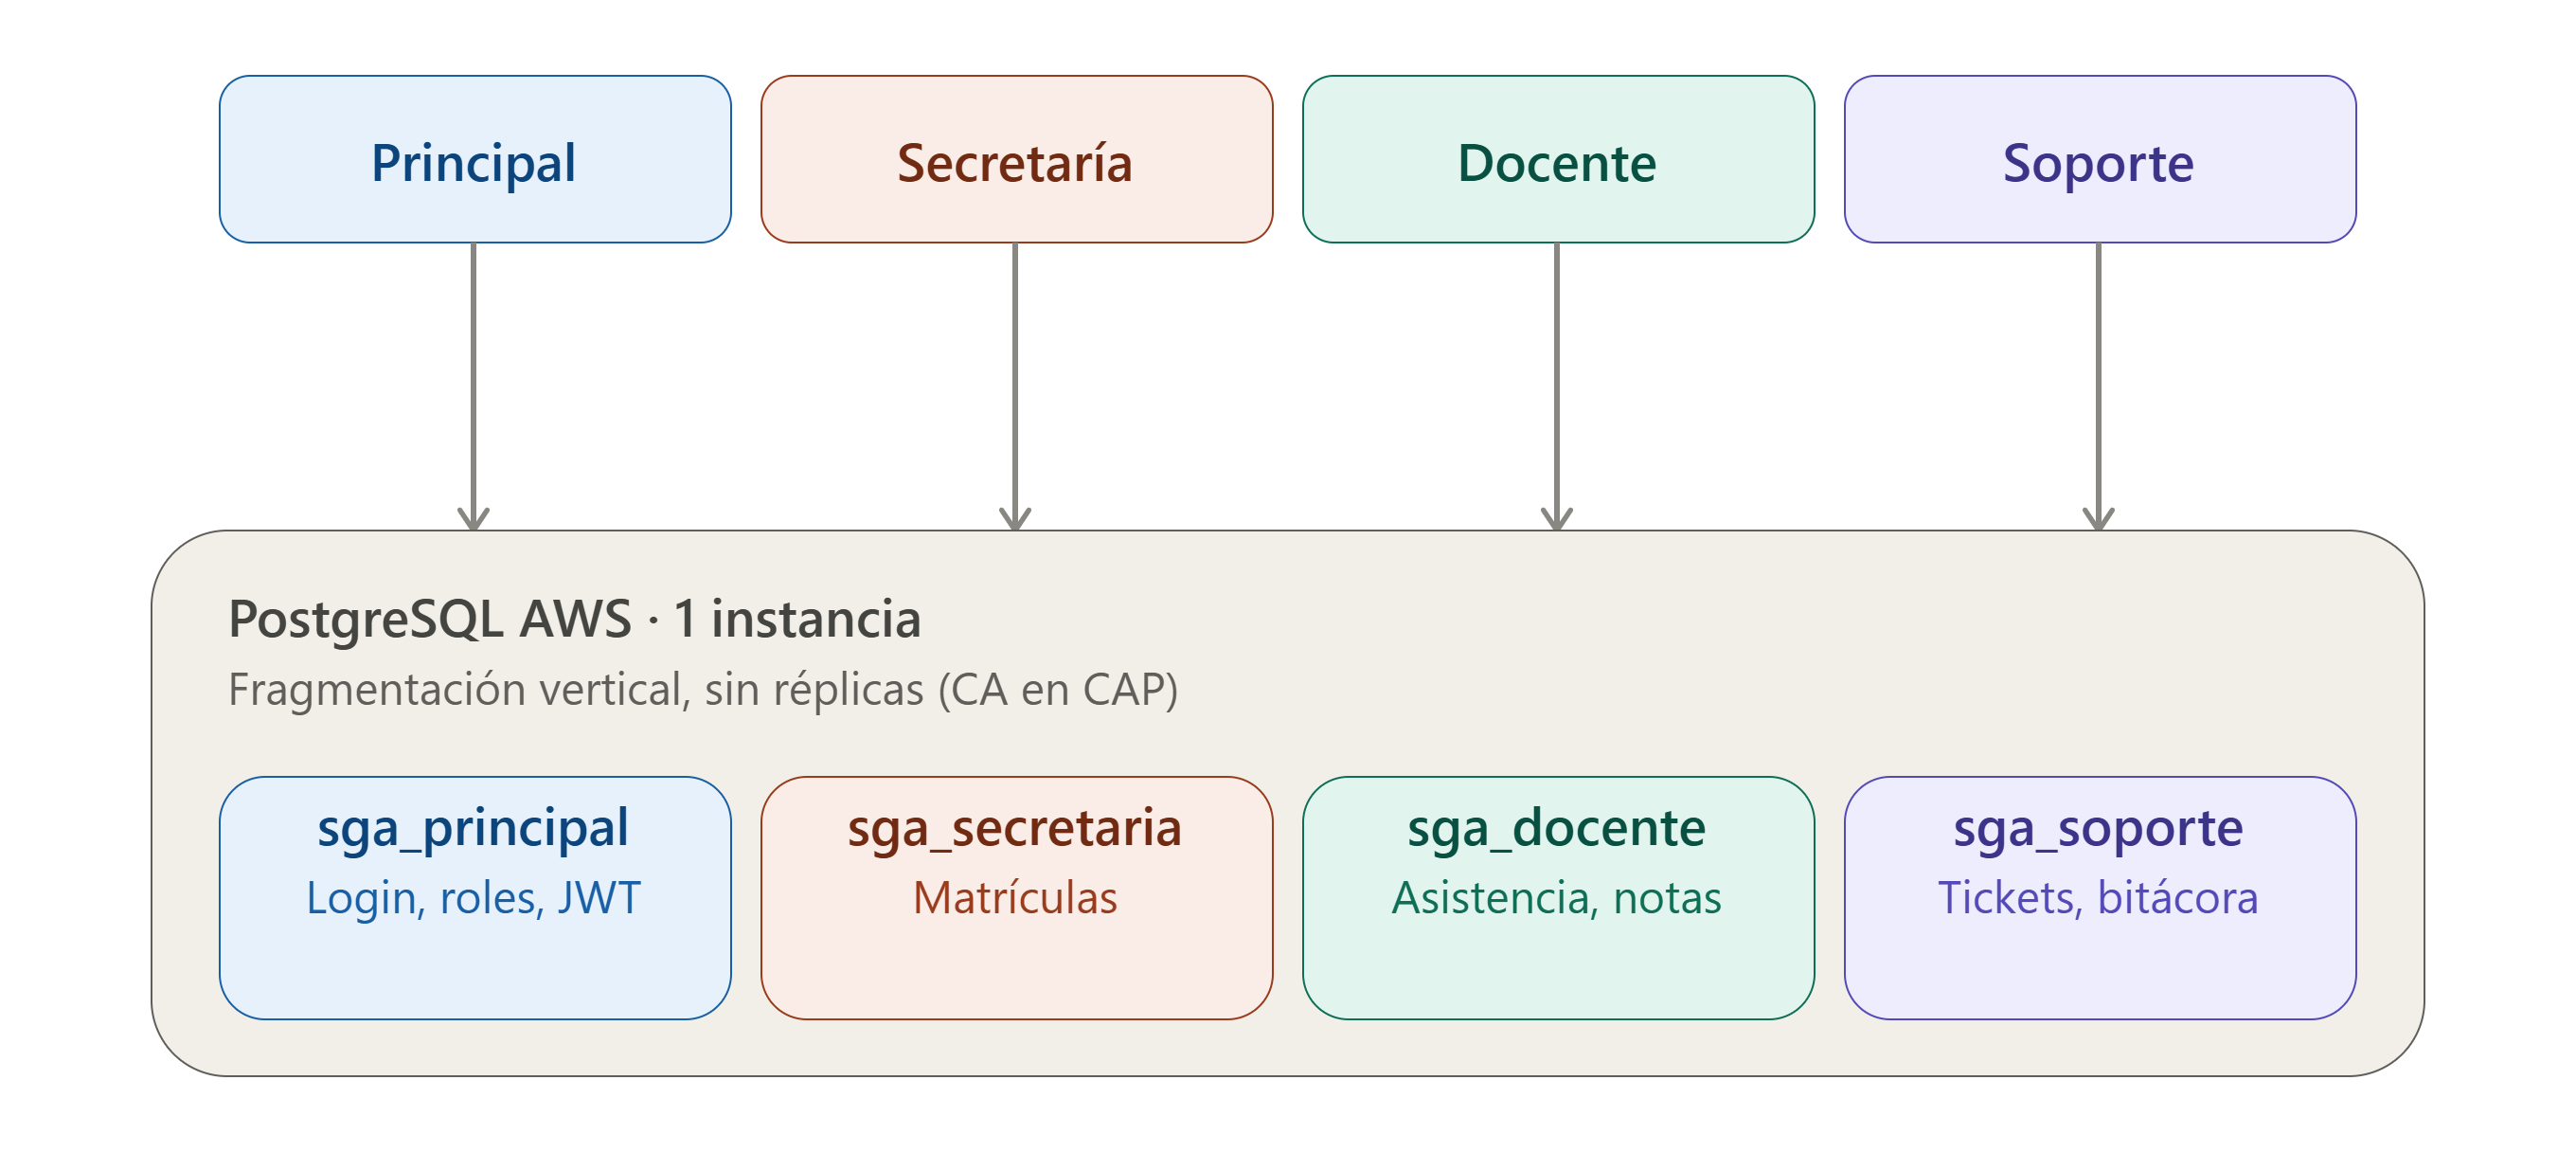
\includegraphics[width=0.85\textwidth]{esquema_distribuido_sga.png}
  \caption{Esquema distribuido efectivamente implementado en E3: cuatro
  microservicios contra una única instancia PostgreSQL en AWS, fragmentada
  verticalmente en cuatro esquemas independientes por servicio.}
  \label{fig:esquema-distribuido}
\end{figure}

Esta estrategia cumple parcialmente las reglas de corrección de
Özsu y Valduriez~\cite{ozsu2020principles}: la \emph{disjunción} se
satisface de forma trivial (cada tabla pertenece a exactamente un esquema,
sin solapamiento), y la \emph{completitud} y \emph{reconstrucción} se
satisfacen a nivel de esquema completo. Sin embargo, esta fragmentación
\textbf{no} es la fragmentación horizontal exigida por el Módulo~B de la
guía: ninguna tabla individual (por ejemplo, \texttt{calificaciones}) fue
particionada en fragmentos $R_1,\dots,R_n$ por un predicado como
\texttt{id\_periodo}; toda la tabla reside íntegra en el esquema
\texttt{sga\_docente} de un único nodo físico. En consecuencia, tampoco se
aplicó colocalización explícita ni factor de replicación $f>1$: el sistema
opera con $f=1$ (Sección~\ref{sec:fundamento-cap}).

\subsection{Registro de decisión arquitectónica (ADR-003)}

Siguiendo la plantilla de Nygard exigida por el Módulo~B, se documenta la
decisión efectivamente tomada:

\begin{quote}
\textbf{ADR-003 --- Fragmentación vertical por microservicio (E3).}\\
\textbf{Estado:} aceptada para E3; superada por ADR-005 (fragmentación
horizontal con CockroachDB) planificada para E4.\\
\textbf{Contexto:} la guía de E3 exige un clúster distribuido con
fragmentación horizontal y consenso; el equipo, por restricciones de
tiempo, priorizó consolidar el contrato \texttt{gRPC} y la autenticación
\texttt{JWT} de \emph{single sign-on} entre los cuatro portales antes de
abordar la migración de persistencia.\\
\textbf{Decisión:} mantener una única instancia PostgreSQL en AWS EC2,
fragmentada verticalmente en cuatro esquemas por servicio, con
\texttt{sga-principal} como único escritor de \texttt{sga\_secretaria}.\\
\textbf{Consecuencias:} (+) aislamiento lógico real de los datos de cada
servicio sin multiplicar infraestructura; (+) migración de esquema
simplificada al no requerir reparto de datos entre nodos; ($-$) persiste el
punto único de falla identificado desde E2 (Sección~\ref{sec:fundamento-cap});
($-$) ninguna tabla individual está fragmentada horizontalmente, por lo que
las consultas de agregación por período siguen ejecutándose sobre el
conjunto completo de la tabla en un solo nodo.
\end{quote}

\subsection{Seguridad de credenciales}

De forma complementaria a la fragmentación, el equipo endureció el manejo
de credenciales en los cuatro esquemas: las contraseñas se almacenan con
\texttt{BCrypt} (costo 10)~\cite{provos1999bcrypt} en lugar de texto plano
en cualquiera de los esquemas, y se exige cambio de contraseña obligatorio
en el primer ingreso de cada usuario --- una medida de higiene de seguridad
independiente de la estrategia de fragmentación, pero relevante para la
integridad del dominio distribuido en su conjunto.


\section{Verificación experimental de la arquitectura implementada}
\label{sec:verificacion-grpc}

Esta sección sustituye al Módulo~C/D de la guía (despliegue y verificación
de tolerancia a fallos de un clúster CockroachDB de tres nodos), que
\textbf{no se ejecutó} porque el clúster correspondiente no fue desplegado
(Sección~\ref{sec:discusion}). En su lugar, se documenta la verificación
que sí se realizó sobre la pieza que efectivamente se consolidó en E3: el
contrato \texttt{gRPC} compartido y la autenticación \texttt{JWT} de
\emph{single sign-on}.

\subsection{Contrato gRPC compartido}

El contrato \texttt{DocenteService} se define en un único archivo
\texttt{docente.proto}, compilado tanto para el cliente Java
(\texttt{sga-principal}) como para el servidor Python (\texttt{micro-docente},
vía \texttt{grpcio}), garantizando que ambos lados del contrato queden
tipados desde la misma fuente:

\begin{lstlisting}[style=codigo,language=Java,caption={Extracto de \texttt{docente.proto}: contrato compartido entre \texttt{sga-principal} (cliente) y \texttt{micro-docente} (servidor).}]
service DocenteService {
  rpc ObtenerCalificaciones (ObtenerCalificacionesRequest)
      returns (ObtenerCalificacionesResponse);
  rpc CalcularPromedioFormativo (PromedioRequest)
      returns (PromedioResponse);
  rpc CalcularPromedioFinal (PromedioRequest)
      returns (PromedioResponse);
  rpc RegistrarCalificacion (RegistrarCalificacionRequest)
      returns (RegistrarCalificacionResponse);
  rpc ConvertirACualitativa (ConvertirACualitativaRequest)
      returns (ConvertirACualitativaResponse);
}

message Calificacion {
  int64 id_calificacion = 1;
  int64 id_actividad = 2;
  int64 id_matricula = 3;
  double nota = 4;
  string nota_cualitativa = 5;
  int32 registrado_por = 6;
}
\end{lstlisting}

El canal \texttt{gRPC} opera en los puertos 9091/9092, separado del canal
\texttt{REST} de \texttt{micro-docente} (puerto 8081), lo que permite
verificar su independencia (Sección~\ref{sec:prueba-independencia}).

\subsection{Autenticación JWT de single sign-on}

El token \texttt{JWT}, firmado con \texttt{HMAC-SHA256} por
\texttt{sga-principal} siguiendo RFC~7519~\cite{jones2015jwt}, se valida en
los cuatro portales (Principal, Secretaría, Docente y Soporte) sin que el
usuario deba autenticarse de nuevo al cambiar de portal. Se verificó
manualmente que un mismo token, obtenido en el login del portal Docente,
es aceptado por los cuatro backends dentro de su ventana de expiración.

\subsection{Prueba de independencia del canal gRPC respecto de la API REST}
\label{sec:prueba-independencia}

Para verificar la afirmación del Resumen (Sección~\ref{sec:resumen}) de que
el canal \texttt{gRPC} opera de forma independiente de la disponibilidad de
la API \texttt{REST} de \texttt{micro-docente}, se siguió el siguiente
procedimiento:

\begin{enumerate}
  \item Con el sistema completo desplegado vía \texttt{docker compose},
        se inicia sesión como docente y se navega al módulo de asistencia
        (portal React en \texttt{localhost:3000}), confirmando que las
        peticiones de negocio (registro de asistencia) viajan por
        \texttt{gRPC} y no por la API \texttt{REST} de Django.
  \item Se detiene únicamente el proceso \texttt{REST} de
        \texttt{micro-docente} (Django Rest Framework), dejando el
        servidor \texttt{gRPC} (\texttt{grpcio}) activo en el mismo
        contenedor.
  \item Se repite el registro de asistencia grupal desde
        \texttt{sga-principal}: la operación se completa con éxito,
        confirmando que el flujo

        \flujo{React $\to$ sga-principal $\to$ gRPC $\to$ micro-docente $\to$ BD}

        \noindent no depende de la disponibilidad de la capa \texttt{REST}.
  \item Se consulta directamente el esquema \texttt{sga\_docente} y se
        confirma la persistencia de las 20 filas de asistencia
        correspondientes al curso de prueba (Figura~\ref{fig:evidencia-asistencia}).
\end{enumerate}

\begin{figure}[H]
  \centering
  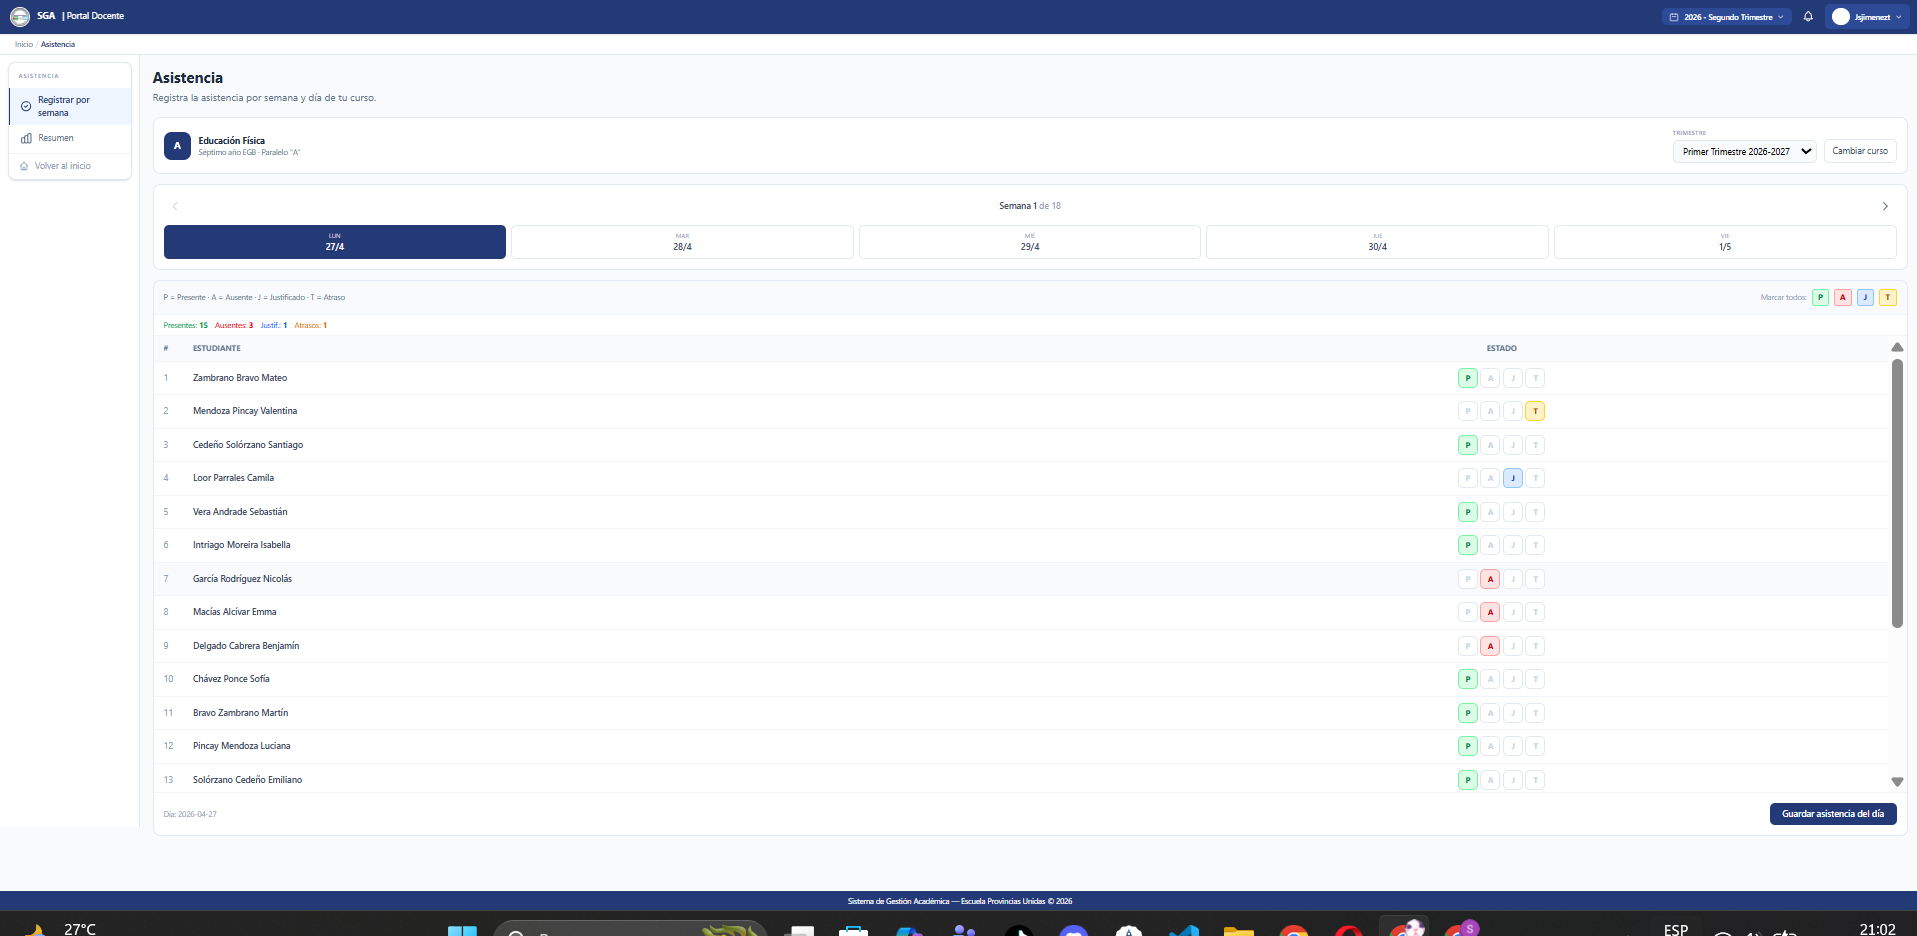
\includegraphics[width=0.85\textwidth]{evidencia_asistencia_docente.png}
  \caption{Portal Docente: registro de asistencia por semana para el curso
  de Educación Física (Séptimo año EGB, Paralelo ``A''), con el conteo de
  presentes, ausentes, justificados y atrasos calculado en tiempo real.}
  \label{fig:evidencia-asistencia}
\end{figure}

Esta prueba corresponde, en alcance, a una verificación de \emph{tolerancia
a fallos de un componente de aplicación} (la API REST), y no
reemplaza la verificación de tolerancia a fallos de \emph{nodos de base de
datos} exigida por el Módulo~D sobre el clúster CockroachDB, que no fue
posible ejecutar al no existir dicho clúster.

% NOTA: subir las capturas reales (login docente, selector de curso,
% marcado P/A/J/T y vista gRPC desde sga-principal) al proyecto de Overleaf
% y descomentar/ajustar el bloque de figura siguiente con el nombre de
% archivo correcto.
%
% \begin{figure}[h]
%   \centering
%   \includegraphics[width=0.8\textwidth]{evidencia_asistencia.png}
%   \caption{Registro de asistencia grupal (20 estudiantes) confirmado en
%   el esquema \texttt{sga\_docente} tras la caída del proceso REST de
%   \texttt{micro-docente}.}
%   \label{fig:evidencia-asistencia}
% \end{figure}


\section{Pipeline analítico paralelo}
\label{sec:pipeline-paralelo}

El Módulo~E de la guía exige un pipeline \texttt{PySpark} con al menos
cinco transformaciones (filtrado, \emph{join} entre tablas colocalizadas,
agregación con ventanas, transformación de tipos temporales y una operación
de \texttt{ml}) sobre datos extraídos del clúster distribuido, junto con un
baseline secuencial en \texttt{pandas} para el contraste de la Ley de
Amdahl. \textbf{Este componente no fue implementado en E3.}

La razón es directa: el pipeline analítico está diseñado para leer, vía
conector JDBC particionado, un clúster con fragmentación horizontal real
(Sección~\ref{sec:fundamento-bdd}); al no existir ese clúster
(Sección~\ref{sec:esquema-distribuido}), el equipo decidió no construir un
pipeline \texttt{Spark} sobre la instancia única de PostgreSQL, ya que
hacerlo habría medido el comportamiento de Spark contra un origen de datos
no representativo del escenario que la guía busca evaluar (rendimiento del
procesamiento paralelo frente a fragmentación real de los datos), y hubiera
requerido rehacer la extracción una vez migrado el clúster en E4.

Se planifica para la Entrega~4 --- una vez desplegado el clúster
CockroachDB de la Sección~\ref{sec:esquema-distribuido} --- implementar
\texttt{spark/pipeline.py} y \texttt{spark/baseline.py} siguiendo el
esqueleto sugerido por la guía, aplicado sobre la tabla
\texttt{calificaciones} con las cinco transformaciones exigidas y el
protocolo experimental completo de la Sección~\ref{sec:protocolo-resultados}.


\section{Protocolo y resultados}
\label{sec:protocolo-resultados}

\subsection{Alcance de la medición realizada}

A diferencia del protocolo estadístico completo del Módulo~F (variable
independiente $N\in\{1,2,4,8\}$ núcleos de Spark, $r=10$ repeticiones por
nivel, intervalo de confianza al 95\,\%), que depende del pipeline
\texttt{PySpark} descrito en la Sección~\ref{sec:pipeline-paralelo} y por
tanto no pudo ejecutarse, el equipo sí realizó una medición comparativa
--- de alcance más acotado --- entre las rutas \texttt{gRPC} y
\texttt{REST} para las dos operaciones más frecuentes del dominio docente.
Esta medición se reporta a continuación con la caveat explícita de que
\textbf{no} sigue el diseño de bloque completo con $r=10$ repeticiones ni
reporta desviación típica o intervalo de confianza; es una medición
preliminar de tiempo de respuesta observado, no un experimento controlado
en el sentido de Wohlin et al.~\cite{wohlin2012experimentation}.

\subsection{Resultados observados}

\begin{table}[h]
  \centering
  \caption{Latencia observada por operación y ruta de comunicación.}
  \label{tab:latencia}
  \begin{tabular}{@{}lcc@{}}
    \toprule
    Operación & Ruta & Latencia observada (ms) \\
    \midrule
    \texttt{RegistrarAsistenciaGrupal} & gRPC & 51 \\
    \texttt{GetMisAsignaciones}        & gRPC & 42 \\
    \texttt{/mis-asignaciones}         & REST & 145 \\
    \bottomrule
  \end{tabular}
\end{table}

Para la operación comparable en ambas rutas, la razón de latencia observada
es de $145/51 \approx 2.8\times$: el canal \texttt{gRPC} respondió
aproximadamente tres veces más rápido que la ruta \texttt{REST} equivalente
en las condiciones de prueba (contenedor local, curso de 20 estudiantes; el
sistema en producción gestiona 677 estudiantes, 13 docentes, 12 grados y 3
paralelos). Esta diferencia es consistente con la literatura sobre
serialización binaria \texttt{Protobuf} frente a \texttt{JSON} sobre
\texttt{HTTP/1.1}~\cite{fielding2000architectural}, aunque --- se insiste
--- no se controlaron aquí variables como el calentamiento de la JVM, el
ruido del sistema anfitrión ni la caché del sistema operativo, que sí
exige el protocolo del Módulo~F para resultados defendibles como evidencia
estadística.

\subsection{Protocolo formal pendiente}

El protocolo completo --- hipótesis $H_1$ vs.\ $H_0$, $r=10$ repeticiones
descartando calentamiento y enfriamiento, prueba $t$ pareada o Wilcoxon
según normalidad, intervalo de confianza al 95\,\% --- queda pendiente y se
aplicará en E4 tanto al pipeline \texttt{Spark} (Sección~\ref{sec:pipeline-paralelo})
como, de forma extendida, a la comparación \texttt{gRPC} vs.\ \texttt{REST}
reportada aquí de forma preliminar. Para esta última, el equipo planea
adoptar además una metodología de \emph{benchmarking} de servicios más
cercana a la de Cooper et al.~\cite{cooper2010ycsb}, generando carga
sintética creciente sobre ambas rutas en lugar de una única medición
puntual por operación.


\section{Discusión}
\label{sec:discusion}

Esta sección discute los resultados reportados siguiendo las
recomendaciones de reporte de estudios de caso en ingeniería de software de
Runeson y Höst~\cite{runeson2009guidelines}: se separan explícitamente las
limitaciones de alcance (qué no se implementó), las amenazas a la validez
de lo que sí se midió, y la relación de continuidad con la entrega
anterior, en lugar de presentar los hallazgos como un experimento cerrado.

\subsection{Limitaciones de esta entrega}

Esta entrega presenta cuatro limitaciones explícitas frente a lo exigido
por la guía de la asignatura:

\begin{enumerate}
  \item \textbf{Ausencia de fragmentación horizontal.} La persistencia
        permanece fragmentada únicamente de forma vertical
        (Sección~\ref{sec:esquema-distribuido}); ninguna tabla fue
        particionada por \texttt{id\_periodo} ni colocalizada por
        \texttt{id\_estudiante}.
  \item \textbf{Ausencia de replicación y consenso.} No se desplegó el
        clúster CockroachDB de tres nodos exigido por el Módulo~C; el
        sistema opera con factor de replicación $f=1$ y, por tanto, sin
        tolerancia a la caída del nodo de base de datos
        (Sección~\ref{sec:fundamento-cap}).
  \item \textbf{Ausencia del pipeline analítico paralelo.} No se
        implementó el pipeline \texttt{PySpark} del Módulo~E
        (Sección~\ref{sec:pipeline-paralelo}), y en consecuencia tampoco
        se dispone de mediciones propias de speedup para contrastar las
        leyes de Amdahl y Gustafson (Sección~\ref{sec:fundamento-spark}).
  \item \textbf{Protocolo experimental incompleto.} La única medición
        cuantitativa reportada (Sección~\ref{sec:protocolo-resultados})
        no sigue el diseño de bloque completo ni reporta intervalos de
        confianza, por lo que debe leerse como indicativa y no como
        evidencia estadísticamente rigurosa.
\end{enumerate}

\subsection{Amenazas a la validez}

\textbf{Internas.} (i) La medición de latencia de la Tabla~\ref{tab:latencia}
se realizó sin repeticiones controladas ni descarte de calentamiento, por
lo que puede estar sesgada por el estado transitorio de la JVM o del
intérprete Python en el momento de la prueba. (ii) La prueba de
independencia \texttt{gRPC}/\texttt{REST} (Sección~\ref{sec:prueba-independencia})
se ejecutó una sola vez de forma manual, sin automatización que garantice
reproducibilidad exacta. (iii) El entorno de prueba corrió en un único
host de desarrollo, sin aislamiento de recursos frente a otros procesos
del sistema anfitrión.

\textbf{Externas.} (i) Los resultados de latencia se midieron sobre un
curso de 20 estudiantes; no está garantizado que la razón
\texttt{gRPC}/\texttt{REST} observada se mantenga con cargas mayores (por
ejemplo, matrícula completa de 677 estudiantes). (ii) El comportamiento
observado corresponde a un entorno de contenedores locales sobre una única
máquina; no se ha probado bajo latencia de red real entre nodos distintos,
condición que sí aplicará una vez desplegado el clúster CockroachDB
distribuido geográfica o físicamente en E4.

\subsection{Relación con la Entrega 2}

La decisión de priorizar la capa de comunicación (\texttt{gRPC}+\texttt{JWT})
sobre la capa de persistencia distribuida es coherente con el estado
heredado de E2: en E2 la comunicación entre procesos ya estaba prototipada
pero no verificada bajo fallos parciales, mientras que la persistencia
mono-nodo, aunque señalada como limitación, seguía siendo funcional para
la demostración de negocio. El equipo optó por cerrar primero la pieza que
condicionaba la usabilidad demostrable del sistema (SSO real entre los
cuatro portales) antes de abordar una migración de base de datos que, de
quedar a medio hacer, habría dejado el sistema completo inoperable para la
defensa oral.


\section{Conclusiones e integración con Entrega 4}
\label{sec:conclusiones}

Este trabajo consolidó y verificó experimentalmente la capa de
comunicación distribuida entre los cuatro microservicios del SGA: un
contrato \texttt{gRPC} compartido entre \texttt{sga-principal} y
\texttt{micro-docente}, autenticación \texttt{JWT} de \emph{single
sign-on} válida en los cuatro portales, e independencia verificada del
canal \texttt{gRPC} respecto de la disponibilidad de la API \texttt{REST}
de docente. La medición preliminar de latencia (Tabla~\ref{tab:latencia})
sugiere una ventaja de aproximadamente $2.8\times$ de \texttt{gRPC} sobre
\texttt{REST} para la operación más frecuente del dominio, aunque esta
cifra debe confirmarse con el protocolo estadístico formal del Módulo~F.

En contraste, este trabajo \textbf{no} alcanzó los dos componentes que la
guía identifica como núcleo de la Entrega~3: un clúster distribuido con
fragmentación horizontal, replicación y consenso (CockroachDB/Raft), y un
pipeline analítico paralelo en Apache Spark contrastado contra las leyes de
Amdahl y Gustafson. Ambos se documentan aquí como limitaciones explícitas
(Sección~\ref{sec:discusion}) y constituyen la prioridad de la Entrega~4.

Los artefactos de esta entrega que se reutilizarán \textbf{sin
modificación} en E4 son: (i)~el contrato \texttt{docente.proto} y el canal
\texttt{gRPC} 9091/9092; (ii)~el esquema de autenticación \texttt{JWT}
\texttt{HMAC-SHA256} de \emph{single sign-on}; (iii)~los cuatro esquemas
lógicos por servicio (\texttt{sga\_principal}, \texttt{sga\_secretaria},
\texttt{sga\_docente}, \texttt{sga\_soporte}), que se migrarán como
namespaces dentro del clúster CockroachDB sin cambiar su modelo de datos;
y (iv)~el \texttt{docker-compose.yml} base, al que se añadirán los
servicios \texttt{crdb-1..3} y \texttt{crdb-init} descritos en el Módulo~C
de la guía. Sobre esta base, la Entrega~4 debe: desplegar el clúster de
tres nodos y aplicar la fragmentación horizontal por \texttt{id\_periodo};
ejecutar la prueba de tolerancia a fallos con caída controlada de uno y de
dos nodos; implementar el pipeline \texttt{PySpark} con sus cinco
transformaciones y el baseline \texttt{pandas}; y correr el protocolo
experimental completo ($r=10$, IC~95\,\%) tanto sobre el pipeline analítico
como, de forma extendida, sobre la comparación \texttt{gRPC}/\texttt{REST}
iniciada en esta entrega.

\bibliographystyle{ieeetr}
\bibliography{referencias}

\end{document}